\DeclareUnicodeCharacter{041B}{\CYRL}



\documentclass[11pt]{article}

    
    \usepackage{anyfontsize}
    \usepackage[breakable]{tcolorbox}
    \usepackage{parskip} % Stop auto-indenting (to mimic markdown behaviour)
    \usepackage[english,russian]{babel}
    \usepackage{graphicx}
    \usepackage{subcaption}

    % Basic figure setup, for now with no caption control since it's done
    % automatically by Pandoc (which extracts ![](path) syntax from Markdown).
    \usepackage{graphicx}
    % Maintain compatibility with old templates. Remove in nbconvert 6.0
    \let\Oldincludegraphics\includegraphics
    % Ensure that by default, figures have no caption (until we provide a
    % proper Figure object with a Caption API and a way to capture that
    % in the conversion process - todo).
    \usepackage{caption}
    \captionsetup{format=nocaption,aboveskip=0pt,belowskip=0pt}

    \usepackage{float}
    \floatplacement{figure}{H} % forces figures to be placed at the correct location
    \usepackage{xcolor} % Allow colors to be defined
    \usepackage{enumerate} % Needed for markdown enumerations to work
    \usepackage{geometry} % Used to adjust the document margins
    \usepackage{amsmath} % Equations
    \usepackage{amssymb} % Equations
    \usepackage{textcomp} % defines textquotesingle
    % Hack from http://tex.stackexchange.com/a/47451/13684:
    \AtBeginDocument{%
        \def\PYZsq{\textquotesingle}% Upright quotes in Pygmentized code
    }
    \usepackage{upquote} % Upright quotes for verbatim code
    \usepackage{eurosym} % defines \euro

    \usepackage{iftex}
    \ifPDFTeX
        \usepackage[T1]{fontenc}
        \IfFileExists{alphabeta.sty}{
              \usepackage{alphabeta}
          }{
              \usepackage[mathletters]{ucs}
              \usepackage[utf8x]{inputenc}
          }
    \else
        \usepackage{fontspec}
        \usepackage{unicode-math}
    \fi

    \usepackage{fancyvrb} % verbatim replacement that allows latex
    \usepackage{grffile} % extends the file name processing of package graphics
                         % to support a larger range
    \makeatletter % fix for old versions of grffile with XeLaTeX
    \@ifpackagelater{grffile}{2019/11/01}
    {
      % Do nothing on new versions
    }
    {
      \def\Gread@@xetex#1{%
        \IfFileExists{"\Gin@base".bb}%
        {\Gread@eps{\Gin@base.bb}}%
        {\Gread@@xetex@aux#1}%
      }
    }
    \makeatother
    \usepackage[Export]{adjustbox} % Used to constrain images to a maximum size
    \adjustboxset{max size={0.9\linewidth}{0.9\paperheight}}

    % The hyperref package gives us a pdf with properly built
    % internal navigation ('pdf bookmarks' for the table of contents,
    % internal cross-reference links, web links for URLs, etc.)
    \usepackage{hyperref}
    % The default LaTeX title has an obnoxious amount of whitespace. By default,
    % titling removes some of it. It also provides customization options.
    \usepackage{titling}
    \usepackage{longtable} % longtable support required by pandoc >1.10
    \usepackage{booktabs}  % table support for pandoc > 1.12.2
    \usepackage{array}     % table support for pandoc >= 2.11.3
    \usepackage{calc}      % table minipage width calculation for pandoc >= 2.11.1
    \usepackage[inline]{enumitem} % IRkernel/repr support (it uses the enumerate* environment)
    \usepackage[normalem]{ulem} % ulem is needed to support strikethroughs (\sout)
                                % normalem makes italics be italics, not underlines
    \usepackage{mathrsfs}
    

    
    % Colors for the hyperref package
    \definecolor{urlcolor}{rgb}{0,.145,.698}
    \definecolor{linkcolor}{rgb}{.71,0.21,0.01}
    \definecolor{citecolor}{rgb}{.12,.54,.11}

    % ANSI colors
    \definecolor{ansi-black}{HTML}{3E424D}
    \definecolor{ansi-black-intense}{HTML}{282C36}
    \definecolor{ansi-red}{HTML}{E75C58}
    \definecolor{ansi-red-intense}{HTML}{B22B31}
    \definecolor{ansi-green}{HTML}{00A250}
    \definecolor{ansi-green-intense}{HTML}{007427}
    \definecolor{ansi-yellow}{HTML}{DDB62B}
    \definecolor{ansi-yellow-intense}{HTML}{B27D12}
    \definecolor{ansi-blue}{HTML}{208FFB}
    \definecolor{ansi-blue-intense}{HTML}{0065CA}
    \definecolor{ansi-magenta}{HTML}{D160C4}
    \definecolor{ansi-magenta-intense}{HTML}{A03196}
    \definecolor{ansi-cyan}{HTML}{60C6C8}
    \definecolor{ansi-cyan-intense}{HTML}{258F8F}
    \definecolor{ansi-white}{HTML}{C5C1B4}
    \definecolor{ansi-white-intense}{HTML}{A1A6B2}
    \definecolor{ansi-default-inverse-fg}{HTML}{FFFFFF}
    \definecolor{ansi-default-inverse-bg}{HTML}{000000}

    % common color for the border for error outputs.
    \definecolor{outerrorbackground}{HTML}{FFDFDF}

    % commands and environments needed by pandoc snippets
    % extracted from the output of `pandoc -s`
    \providecommand{\tightlist}{%
      \setlength{\itemsep}{0pt}\setlength{\parskip}{0pt}}
    \DefineVerbatimEnvironment{Highlighting}{Verbatim}{commandchars=\\\{\}}
    % Add ',fontsize=\small' for more characters per line
    \newenvironment{Shaded}{}{}
    \newcommand{\KeywordTok}[1]{\textcolor[rgb]{0.00,0.44,0.13}{\textbf{{#1}}}}
    \newcommand{\DataTypeTok}[1]{\textcolor[rgb]{0.56,0.13,0.00}{{#1}}}
    \newcommand{\DecValTok}[1]{\textcolor[rgb]{0.25,0.63,0.44}{{#1}}}
    \newcommand{\BaseNTok}[1]{\textcolor[rgb]{0.25,0.63,0.44}{{#1}}}
    \newcommand{\FloatTok}[1]{\textcolor[rgb]{0.25,0.63,0.44}{{#1}}}
    \newcommand{\CharTok}[1]{\textcolor[rgb]{0.25,0.44,0.63}{{#1}}}
    \newcommand{\StringTok}[1]{\textcolor[rgb]{0.25,0.44,0.63}{{#1}}}
    \newcommand{\CommentTok}[1]{\textcolor[rgb]{0.38,0.63,0.69}{\textit{{#1}}}}
    \newcommand{\OtherTok}[1]{\textcolor[rgb]{0.00,0.44,0.13}{{#1}}}
    \newcommand{\AlertTok}[1]{\textcolor[rgb]{1.00,0.00,0.00}{\textbf{{#1}}}}
    \newcommand{\FunctionTok}[1]{\textcolor[rgb]{0.02,0.16,0.49}{{#1}}}
    \newcommand{\RegionMarkerTok}[1]{{#1}}
    \newcommand{\ErrorTok}[1]{\textcolor[rgb]{1.00,0.00,0.00}{\textbf{{#1}}}}
    \newcommand{\NormalTok}[1]{{#1}}

    % Additional commands for more recent versions of Pandoc
    \newcommand{\ConstantTok}[1]{\textcolor[rgb]{0.53,0.00,0.00}{{#1}}}
    \newcommand{\SpecialCharTok}[1]{\textcolor[rgb]{0.25,0.44,0.63}{{#1}}}
    \newcommand{\VerbatimStringTok}[1]{\textcolor[rgb]{0.25,0.44,0.63}{{#1}}}
    \newcommand{\SpecialStringTok}[1]{\textcolor[rgb]{0.73,0.40,0.53}{{#1}}}
    \newcommand{\ImportTok}[1]{{#1}}
    \newcommand{\DocumentationTok}[1]{\textcolor[rgb]{0.73,0.13,0.13}{\textit{{#1}}}}
    \newcommand{\AnnotationTok}[1]{\textcolor[rgb]{0.38,0.63,0.69}{\textbf{\textit{{#1}}}}}
    \newcommand{\CommentVarTok}[1]{\textcolor[rgb]{0.38,0.63,0.69}{\textbf{\textit{{#1}}}}}
    \newcommand{\VariableTok}[1]{\textcolor[rgb]{0.10,0.09,0.49}{{#1}}}
    \newcommand{\ControlFlowTok}[1]{\textcolor[rgb]{0.00,0.44,0.13}{\textbf{{#1}}}}
    \newcommand{\OperatorTok}[1]{\textcolor[rgb]{0.40,0.40,0.40}{{#1}}}
    \newcommand{\BuiltInTok}[1]{{#1}}
    \newcommand{\ExtensionTok}[1]{{#1}}
    \newcommand{\PreprocessorTok}[1]{\textcolor[rgb]{0.74,0.48,0.00}{{#1}}}
    \newcommand{\AttributeTok}[1]{\textcolor[rgb]{0.49,0.56,0.16}{{#1}}}
    \newcommand{\InformationTok}[1]{\textcolor[rgb]{0.38,0.63,0.69}{\textbf{\textit{{#1}}}}}
    \newcommand{\WarningTok}[1]{\textcolor[rgb]{0.38,0.63,0.69}{\textbf{\textit{{#1}}}}}


    % Define a nice break command that doesn't care if a line doesn't already
    % exist.
    \def\br{\hspace*{\fill} \\* }
    % Math Jax compatibility definitions
    \def\gt{>}
    \def\lt{<}
    \let\Oldtex\TeX
    \let\Oldlatex\LaTeX
    \renewcommand{\TeX}{\textrm{\Oldtex}}
    \renewcommand{\LaTeX}{\textrm{\Oldlatex}}
    % Document parameters
    % Document title
    \title{Лабораторная работа номер 3. \\ Предварительный, корреляционный и регрессионный анализ неоднородных данных }
    \author{Карпович Артём Дмитриевич. 7 группа}
    
    
    
    
    
% Pygments definitions
\makeatletter
\def\PY@reset{\let\PY@it=\relax \let\PY@bf=\relax%
    \let\PY@ul=\relax \let\PY@tc=\relax%
    \let\PY@bc=\relax \let\PY@ff=\relax}
\def\PY@tok#1{\csname PY@tok@#1\endcsname}
\def\PY@toks#1+{\ifx\relax#1\empty\else%
    \PY@tok{#1}\expandafter\PY@toks\fi}
\def\PY@do#1{\PY@bc{\PY@tc{\PY@ul{%
    \PY@it{\PY@bf{\PY@ff{#1}}}}}}}
\def\PY#1#2{\PY@reset\PY@toks#1+\relax+\PY@do{#2}}

\@namedef{PY@tok@w}{\def\PY@tc##1{\textcolor[rgb]{0.73,0.73,0.73}{##1}}}
\@namedef{PY@tok@c}{\let\PY@it=\textit\def\PY@tc##1{\textcolor[rgb]{0.24,0.48,0.48}{##1}}}
\@namedef{PY@tok@cp}{\def\PY@tc##1{\textcolor[rgb]{0.61,0.40,0.00}{##1}}}
\@namedef{PY@tok@k}{\let\PY@bf=\textbf\def\PY@tc##1{\textcolor[rgb]{0.00,0.50,0.00}{##1}}}
\@namedef{PY@tok@kp}{\def\PY@tc##1{\textcolor[rgb]{0.00,0.50,0.00}{##1}}}
\@namedef{PY@tok@kt}{\def\PY@tc##1{\textcolor[rgb]{0.69,0.00,0.25}{##1}}}
\@namedef{PY@tok@o}{\def\PY@tc##1{\textcolor[rgb]{0.40,0.40,0.40}{##1}}}
\@namedef{PY@tok@ow}{\let\PY@bf=\textbf\def\PY@tc##1{\textcolor[rgb]{0.67,0.13,1.00}{##1}}}
\@namedef{PY@tok@nb}{\def\PY@tc##1{\textcolor[rgb]{0.00,0.50,0.00}{##1}}}
\@namedef{PY@tok@nf}{\def\PY@tc##1{\textcolor[rgb]{0.00,0.00,1.00}{##1}}}
\@namedef{PY@tok@nc}{\let\PY@bf=\textbf\def\PY@tc##1{\textcolor[rgb]{0.00,0.00,1.00}{##1}}}
\@namedef{PY@tok@nn}{\let\PY@bf=\textbf\def\PY@tc##1{\textcolor[rgb]{0.00,0.00,1.00}{##1}}}
\@namedef{PY@tok@ne}{\let\PY@bf=\textbf\def\PY@tc##1{\textcolor[rgb]{0.80,0.25,0.22}{##1}}}
\@namedef{PY@tok@nv}{\def\PY@tc##1{\textcolor[rgb]{0.10,0.09,0.49}{##1}}}
\@namedef{PY@tok@no}{\def\PY@tc##1{\textcolor[rgb]{0.53,0.00,0.00}{##1}}}
\@namedef{PY@tok@nl}{\def\PY@tc##1{\textcolor[rgb]{0.46,0.46,0.00}{##1}}}
\@namedef{PY@tok@ni}{\let\PY@bf=\textbf\def\PY@tc##1{\textcolor[rgb]{0.44,0.44,0.44}{##1}}}
\@namedef{PY@tok@na}{\def\PY@tc##1{\textcolor[rgb]{0.41,0.47,0.13}{##1}}}
\@namedef{PY@tok@nt}{\let\PY@bf=\textbf\def\PY@tc##1{\textcolor[rgb]{0.00,0.50,0.00}{##1}}}
\@namedef{PY@tok@nd}{\def\PY@tc##1{\textcolor[rgb]{0.67,0.13,1.00}{##1}}}
\@namedef{PY@tok@s}{\def\PY@tc##1{\textcolor[rgb]{0.73,0.13,0.13}{##1}}}
\@namedef{PY@tok@sd}{\let\PY@it=\textit\def\PY@tc##1{\textcolor[rgb]{0.73,0.13,0.13}{##1}}}
\@namedef{PY@tok@si}{\let\PY@bf=\textbf\def\PY@tc##1{\textcolor[rgb]{0.64,0.35,0.47}{##1}}}
\@namedef{PY@tok@se}{\let\PY@bf=\textbf\def\PY@tc##1{\textcolor[rgb]{0.67,0.36,0.12}{##1}}}
\@namedef{PY@tok@sr}{\def\PY@tc##1{\textcolor[rgb]{0.64,0.35,0.47}{##1}}}
\@namedef{PY@tok@ss}{\def\PY@tc##1{\textcolor[rgb]{0.10,0.09,0.49}{##1}}}
\@namedef{PY@tok@sx}{\def\PY@tc##1{\textcolor[rgb]{0.00,0.50,0.00}{##1}}}
\@namedef{PY@tok@m}{\def\PY@tc##1{\textcolor[rgb]{0.40,0.40,0.40}{##1}}}
\@namedef{PY@tok@gh}{\let\PY@bf=\textbf\def\PY@tc##1{\textcolor[rgb]{0.00,0.00,0.50}{##1}}}
\@namedef{PY@tok@gu}{\let\PY@bf=\textbf\def\PY@tc##1{\textcolor[rgb]{0.50,0.00,0.50}{##1}}}
\@namedef{PY@tok@gd}{\def\PY@tc##1{\textcolor[rgb]{0.63,0.00,0.00}{##1}}}
\@namedef{PY@tok@gi}{\def\PY@tc##1{\textcolor[rgb]{0.00,0.52,0.00}{##1}}}
\@namedef{PY@tok@gr}{\def\PY@tc##1{\textcolor[rgb]{0.89,0.00,0.00}{##1}}}
\@namedef{PY@tok@ge}{\let\PY@it=\textit}
\@namedef{PY@tok@gs}{\let\PY@bf=\textbf}
\@namedef{PY@tok@gp}{\let\PY@bf=\textbf\def\PY@tc##1{\textcolor[rgb]{0.00,0.00,0.50}{##1}}}
\@namedef{PY@tok@go}{\def\PY@tc##1{\textcolor[rgb]{0.44,0.44,0.44}{##1}}}
\@namedef{PY@tok@gt}{\def\PY@tc##1{\textcolor[rgb]{0.00,0.27,0.87}{##1}}}
\@namedef{PY@tok@err}{\def\PY@bc##1{{\setlength{\fboxsep}{\string -\fboxrule}\fcolorbox[rgb]{1.00,0.00,0.00}{1,1,1}{\strut ##1}}}}
\@namedef{PY@tok@kc}{\let\PY@bf=\textbf\def\PY@tc##1{\textcolor[rgb]{0.00,0.50,0.00}{##1}}}
\@namedef{PY@tok@kd}{\let\PY@bf=\textbf\def\PY@tc##1{\textcolor[rgb]{0.00,0.50,0.00}{##1}}}
\@namedef{PY@tok@kn}{\let\PY@bf=\textbf\def\PY@tc##1{\textcolor[rgb]{0.00,0.50,0.00}{##1}}}
\@namedef{PY@tok@kr}{\let\PY@bf=\textbf\def\PY@tc##1{\textcolor[rgb]{0.00,0.50,0.00}{##1}}}
\@namedef{PY@tok@bp}{\def\PY@tc##1{\textcolor[rgb]{0.00,0.50,0.00}{##1}}}
\@namedef{PY@tok@fm}{\def\PY@tc##1{\textcolor[rgb]{0.00,0.00,1.00}{##1}}}
\@namedef{PY@tok@vc}{\def\PY@tc##1{\textcolor[rgb]{0.10,0.09,0.49}{##1}}}
\@namedef{PY@tok@vg}{\def\PY@tc##1{\textcolor[rgb]{0.10,0.09,0.49}{##1}}}
\@namedef{PY@tok@vi}{\def\PY@tc##1{\textcolor[rgb]{0.10,0.09,0.49}{##1}}}
\@namedef{PY@tok@vm}{\def\PY@tc##1{\textcolor[rgb]{0.10,0.09,0.49}{##1}}}
\@namedef{PY@tok@sa}{\def\PY@tc##1{\textcolor[rgb]{0.73,0.13,0.13}{##1}}}
\@namedef{PY@tok@sb}{\def\PY@tc##1{\textcolor[rgb]{0.73,0.13,0.13}{##1}}}
\@namedef{PY@tok@sc}{\def\PY@tc##1{\textcolor[rgb]{0.73,0.13,0.13}{##1}}}
\@namedef{PY@tok@dl}{\def\PY@tc##1{\textcolor[rgb]{0.73,0.13,0.13}{##1}}}
\@namedef{PY@tok@s2}{\def\PY@tc##1{\textcolor[rgb]{0.73,0.13,0.13}{##1}}}
\@namedef{PY@tok@sh}{\def\PY@tc##1{\textcolor[rgb]{0.73,0.13,0.13}{##1}}}
\@namedef{PY@tok@s1}{\def\PY@tc##1{\textcolor[rgb]{0.73,0.13,0.13}{##1}}}
\@namedef{PY@tok@mb}{\def\PY@tc##1{\textcolor[rgb]{0.40,0.40,0.40}{##1}}}
\@namedef{PY@tok@mf}{\def\PY@tc##1{\textcolor[rgb]{0.40,0.40,0.40}{##1}}}
\@namedef{PY@tok@mh}{\def\PY@tc##1{\textcolor[rgb]{0.40,0.40,0.40}{##1}}}
\@namedef{PY@tok@mi}{\def\PY@tc##1{\textcolor[rgb]{0.40,0.40,0.40}{##1}}}
\@namedef{PY@tok@il}{\def\PY@tc##1{\textcolor[rgb]{0.40,0.40,0.40}{##1}}}
\@namedef{PY@tok@mo}{\def\PY@tc##1{\textcolor[rgb]{0.40,0.40,0.40}{##1}}}
\@namedef{PY@tok@ch}{\let\PY@it=\textit\def\PY@tc##1{\textcolor[rgb]{0.24,0.48,0.48}{##1}}}
\@namedef{PY@tok@cm}{\let\PY@it=\textit\def\PY@tc##1{\textcolor[rgb]{0.24,0.48,0.48}{##1}}}
\@namedef{PY@tok@cpf}{\let\PY@it=\textit\def\PY@tc##1{\textcolor[rgb]{0.24,0.48,0.48}{##1}}}
\@namedef{PY@tok@c1}{\let\PY@it=\textit\def\PY@tc##1{\textcolor[rgb]{0.24,0.48,0.48}{##1}}}
\@namedef{PY@tok@cs}{\let\PY@it=\textit\def\PY@tc##1{\textcolor[rgb]{0.24,0.48,0.48}{##1}}}

\def\PYZbs{\char`\\}
\def\PYZus{\char`\_}
\def\PYZob{\char`\{}
\def\PYZcb{\char`\}}
\def\PYZca{\char`\^}
\def\PYZam{\char`\&}
\def\PYZlt{\char`\<}
\def\PYZgt{\char`\>}
\def\PYZsh{\char`\#}
\def\PYZpc{\char`\%}
\def\PYZdl{\char`\$}
\def\PYZhy{\char`\-}
\def\PYZsq{\char`\'}
\def\PYZdq{\char`\"}
\def\PYZti{\char`\~}
% for compatibility with earlier versions
\def\PYZat{@}
\def\PYZlb{[}
\def\PYZrb{]}
\makeatother


    % For linebreaks inside Verbatim environment from package fancyvrb.
    \makeatletter
        \newbox\Wrappedcontinuationbox
        \newbox\Wrappedvisiblespacebox
        \newcommand*\Wrappedvisiblespace {\textcolor{red}{\textvisiblespace}}
        \newcommand*\Wrappedcontinuationsymbol {\textcolor{red}{\llap{\tiny$\m@th\hookrightarrow$}}}
        \newcommand*\Wrappedcontinuationindent {3ex }
        \newcommand*\Wrappedafterbreak {\kern\Wrappedcontinuationindent\copy\Wrappedcontinuationbox}
        % Take advantage of the already applied Pygments mark-up to insert
        % potential linebreaks for TeX processing.
        %        {, <, #, %, $, ' and ": go to next line.
        %        _, }, ^, &, >, - and ~: stay at end of broken line.
        % Use of \textquotesingle for straight quote.
        \newcommand*\Wrappedbreaksatspecials {%
            \def\PYGZus{\discretionary{\char`\_}{\Wrappedafterbreak}{\char`\_}}%
            \def\PYGZob{\discretionary{}{\Wrappedafterbreak\char`\{}{\char`\{}}%
            \def\PYGZcb{\discretionary{\char`\}}{\Wrappedafterbreak}{\char`\}}}%
            \def\PYGZca{\discretionary{\char`\^}{\Wrappedafterbreak}{\char`\^}}%
            \def\PYGZam{\discretionary{\char`\&}{\Wrappedafterbreak}{\char`\&}}%
            \def\PYGZlt{\discretionary{}{\Wrappedafterbreak\char`\<}{\char`\<}}%
            \def\PYGZgt{\discretionary{\char`\>}{\Wrappedafterbreak}{\char`\>}}%
            \def\PYGZsh{\discretionary{}{\Wrappedafterbreak\char`\#}{\char`\#}}%
            \def\PYGZpc{\discretionary{}{\Wrappedafterbreak\char`\%}{\char`\%}}%
            \def\PYGZdl{\discretionary{}{\Wrappedafterbreak\char`\$}{\char`\$}}%
            \def\PYGZhy{\discretionary{\char`\-}{\Wrappedafterbreak}{\char`\-}}%
            \def\PYGZsq{\discretionary{}{\Wrappedafterbreak\textquotesingle}{\textquotesingle}}%
            \def\PYGZdq{\discretionary{}{\Wrappedafterbreak\char`\"}{\char`\"}}%
            \def\PYGZti{\discretionary{\char`\~}{\Wrappedafterbreak}{\char`\~}}%
        }
        % Some characters . , ; ? ! / are not pygmentized.
        % This macro makes them "active" and they will insert potential linebreaks
        \newcommand*\Wrappedbreaksatpunct {%
            \lccode`\~`\.\lowercase{\def~}{\discretionary{\hbox{\char`\.}}{\Wrappedafterbreak}{\hbox{\char`\.}}}%
            \lccode`\~`\,\lowercase{\def~}{\discretionary{\hbox{\char`\,}}{\Wrappedafterbreak}{\hbox{\char`\,}}}%
            \lccode`\~`\;\lowercase{\def~}{\discretionary{\hbox{\char`\;}}{\Wrappedafterbreak}{\hbox{\char`\;}}}%
            \lccode`\~`\:\lowercase{\def~}{\discretionary{\hbox{\char`\:}}{\Wrappedafterbreak}{\hbox{\char`\:}}}%
            \lccode`\~`\?\lowercase{\def~}{\discretionary{\hbox{\char`\?}}{\Wrappedafterbreak}{\hbox{\char`\?}}}%
            \lccode`\~`\!\lowercase{\def~}{\discretionary{\hbox{\char`\!}}{\Wrappedafterbreak}{\hbox{\char`\!}}}%
            \lccode`\~`\/\lowercase{\def~}{\discretionary{\hbox{\char`\/}}{\Wrappedafterbreak}{\hbox{\char`\/}}}%
            \catcode`\.\active
            \catcode`\,\active
            \catcode`\;\active
            \catcode`\:\active
            \catcode`\?\active
            \catcode`\!\active
            \catcode`\/\active
            \lccode`\~`\~
        }
    \makeatother

    \let\OriginalVerbatim=\Verbatim
    \makeatletter
    \renewcommand{\Verbatim}[1][1]{%
        %\parskip\z@skip
        \sbox\Wrappedcontinuationbox {\Wrappedcontinuationsymbol}%
        \sbox\Wrappedvisiblespacebox {\FV@SetupFont\Wrappedvisiblespace}%
        \def\FancyVerbFormatLine ##1{\hsize\linewidth
            \vtop{\raggedright\hyphenpenalty\z@\exhyphenpenalty\z@
                \doublehyphendemerits\z@\finalhyphendemerits\z@
                \strut ##1\strut}%
        }%
        % If the linebreak is at a space, the latter will be displayed as visible
        % space at end of first line, and a continuation symbol starts next line.
        % Stretch/shrink are however usually zero for typewriter font.
        \def\FV@Space {%
            \nobreak\hskip\z@ plus\fontdimen3\font minus\fontdimen4\font
            \discretionary{\copy\Wrappedvisiblespacebox}{\Wrappedafterbreak}
            {\kern\fontdimen2\font}%
        }%

        % Allow breaks at special characters using \PYG... macros.
        \Wrappedbreaksatspecials
        % Breaks at punctuation characters . , ; ? ! and / need catcode=\active
        \OriginalVerbatim[#1,codes*=\Wrappedbreaksatpunct]%
    }
    \makeatother

    % Exact colors from NB
    \definecolor{incolor}{HTML}{303F9F}
    \definecolor{outcolor}{HTML}{D84315}
    \definecolor{cellborder}{HTML}{CFCFCF}
    \definecolor{cellbackground}{HTML}{F7F7F7}

    % prompt
    \makeatletter
    \newcommand{\boxspacing}{\kern\kvtcb@left@rule\kern\kvtcb@boxsep}
    \makeatother
    \newcommand{\prompt}[4]{
        {\ttfamily\llap{{\color{#2}[#3]:\hspace{3pt}#4}}\vspace{-\baselineskip}}
    }
    

    
    % Prevent overflowing lines due to hard-to-break entities
    \sloppy
    % Setup hyperref package
    \hypersetup{
      breaklinks=true,  % so long urls are correctly broken across lines
      colorlinks=true,
      urlcolor=urlcolor,
      linkcolor=linkcolor,
      citecolor=citecolor,
      }
    % Slightly bigger margins than the latex defaults
    
    \geometry{verbose,tmargin=1in,bmargin=1in,lmargin=1in,rmargin=1in}
    
    

\begin{document}

    \begin{titlepage}
    \newpage
    
    \begin{center}
    МИНИСТЕРСТВО ОБРАЗОВАНИЯ РЕСПУБЛИКИ БЕЛАРУСЬ БЕЛОРУССКИЙ ГОСУДАРСТВЕННЫЙ УНИВЕРСИТЕТ \\
    Факультет прикладной математики и инворматики \\ Кафедра информационных систем управления 
    \end{center}
    
    \vspace{8em}
    
    \vspace{2em}
    
    \begin{center}
    \textsc{\textbf{Отчет по лабораторной работе 7-8 \linebreak Вариант 5}}
    \end{center}
    
    \vspace{6em}
    
    \begin{flushright}
        Выполнил:\\
        Карпович Артём Дмитриевич\\
        студент 3 курса 7 группы
    \end{flushright}

    \begin{flushright}
        Преподаватель:\\
        Кваша Дарья Юрьевна
    \end{flushright}
    \vspace{\fill}
    
    \begin{center}
    Минск, 2024
    \end{center}
    
    \end{titlepage}
    
    

    
    \begin{center}
        \subsection*{Задачи теории игр}
\end{center}
\subsubsection*{Задача 1}

Найти решение игры, заданной матрицей \(A_5\): \[\begin{bmatrix}
-1 & 3\\
7 & -2
\end{bmatrix}\]

Решением матричной игры в чистых стратегиях называется пара чистых
стратегий \((i_0, j_0)\) первого и второго игроков, которые образуют
седловую точку матрицы \(A\):
\(a_{ij_0} \leq a_{i_0j_0} \leq a_{i_0j} , i = 1, ... , m, j = 1, . . . , n.\)

Решением матричной игры в смешанных стратегиях называют пару смешанных
стратегий \((p_0, q_0)\), которая образует седловую точку функции
\(E_A(p, q),\) т. е.
\[E_A(p, q^0) \leq E_A(p^0, q^0) \leq E_A(p^0, q), p \in \Sigma_m, q \in \Sigma_n.\]

    \begin{tcolorbox}[breakable, size=fbox, boxrule=1pt, pad at break*=1mm,colback=cellbackground, colframe=cellborder]
\prompt{In}{incolor}{1}{\boxspacing}
\begin{Verbatim}[commandchars=\\\{\}]
\PY{k+kn}{import} \PY{n+nn}{numpy} \PY{k}{as} \PY{n+nn}{np}

\PY{n}{A} \PY{o}{=} \PY{n}{np}\PY{o}{.}\PY{n}{array}\PY{p}{(}\PY{p}{[}\PY{p}{[}\PY{o}{\PYZhy{}}\PY{l+m+mi}{1}\PY{p}{,} \PY{l+m+mi}{3}\PY{p}{]}\PY{p}{,}
               \PY{p}{[}\PY{l+m+mi}{7}\PY{p}{,} \PY{o}{\PYZhy{}}\PY{l+m+mi}{2}\PY{p}{]}\PY{p}{]}\PY{p}{)}

\PY{n}{row\PYZus{}min} \PY{o}{=} \PY{n}{np}\PY{o}{.}\PY{n}{min}\PY{p}{(}\PY{n}{A}\PY{p}{,} \PY{n}{axis}\PY{o}{=}\PY{l+m+mi}{1}\PY{p}{)}
\PY{n}{column\PYZus{}max} \PY{o}{=} \PY{n}{np}\PY{o}{.}\PY{n}{max}\PY{p}{(}\PY{n}{A}\PY{p}{,} \PY{n}{axis}\PY{o}{=}\PY{l+m+mi}{0}\PY{p}{)}

\PY{n}{row\PYZus{}min\PYZus{}max} \PY{o}{=} \PY{n}{np}\PY{o}{.}\PY{n}{max}\PY{p}{(}\PY{n}{row\PYZus{}min}\PY{p}{)}
\PY{n}{column\PYZus{}max\PYZus{}min} \PY{o}{=} \PY{n}{np}\PY{o}{.}\PY{n}{min}\PY{p}{(}\PY{n}{column\PYZus{}max}\PY{p}{)}

\PY{k}{if} \PY{n}{row\PYZus{}min\PYZus{}max} \PY{o}{==} \PY{n}{column\PYZus{}max\PYZus{}min}\PY{p}{:}
    \PY{n+nb}{print}\PY{p}{(}\PY{l+s+s2}{\PYZdq{}}\PY{l+s+s2}{Седловая точка найдена: }\PY{l+s+s2}{\PYZdq{}}\PY{p}{,} \PY{n}{row\PYZus{}min\PYZus{}max}\PY{p}{)}
\PY{k}{else}\PY{p}{:}
    \PY{n+nb}{print}\PY{p}{(}\PY{l+s+s2}{\PYZdq{}}\PY{l+s+s2}{Седловая точка не найдена.}\PY{l+s+s2}{\PYZdq{}}\PY{p}{)}
\end{Verbatim}
\end{tcolorbox}

    \begin{Verbatim}[commandchars=\\\{\}]
Седловая точка не найдена.
    \end{Verbatim}

    Результатом стало то, что седловой точки в этой задаче нет, тогда цена
игры находится в пределах \(-1 \leq y \leq 3\). Находим решение игры в
смешанных стратегиях. Объясняется это тем, что игроки не могут объявить
противнику свои чистые стратегии: им следует скрывать свои действия.
Игру можно решить, если позволить игрокам выбирать свои стратегии
случайным образом (смешивать чистые стратегии). Так как игроки выбирают
свои чистые стратегии случайным образом, то выигрыш игрока \(I\) будет
случайной величиной. В этом случае игрок \(I\) должен выбрать свои
смешанные стратегии так, чтобы получить максимальный средний выигрыш.
Аналогично, игрок \(II\) должен выбрать свои смешанные стратегии так,
чтобы минимизировать математическое ожидание игрока \(I\).

Запишем систему уравнений. Для игрока \(I\) \[-p_1+7p_2 = y,\]
 \[3p_1-2p_2 = y,\]  \[p_1+p_2 = 1.\]

Для игрока \(II\) \[-q_1+3q_2 = y,\]  \[7q_1-2q_2 = y,\]
 \[q_1+q_2 = 1.\]

Решая эту систему получим следующее
\[v = \dfrac{19}{13}\ -\ \text{стоимость игры},\]
\[p_1 = \dfrac{9}{13}\ - \ \text{вероятность применения 1-ой стратегии},\]
\[p_2 = \dfrac{4}{13}\ - \ \text{вероятность применения 2-ой стратегии}.\]
Оптимальная смешанная стратегия игрока
\(I: P = (\dfrac{9}{13}; \dfrac{4}{13}).\)
\[q_1 = \dfrac{5}{13}\ - \ \text{вероятность применения 1-ой стратегии},\]
\[q_2 = \dfrac{8}{13}\ - \ \text{вероятность применения 2-ой стратегии}.\]
Оптимальная смешанная стратегия игрока
\(II: Q = (\dfrac{5}{13}; \dfrac{8}{13}).\)

    \subsubsection*{Задача 2}

Найдите решение игр, заданных матрицами \(A_{5, 1}\) и \(A_{5, 2}\):
\[A_{5, 1}=\begin{bmatrix}
4 & 0 & 2 & 1\\
-2 & 5 & -3 & -1
\end{bmatrix} \ 
A_{5, 2} = \begin{bmatrix}
2 & 4 \\
6 & -2 \\
4 & 2
\end{bmatrix}\]

    \begin{tcolorbox}[breakable, size=fbox, boxrule=1pt, pad at break*=1mm,colback=cellbackground, colframe=cellborder]
\prompt{In}{incolor}{18}{\boxspacing}
\begin{Verbatim}[commandchars=\\\{\}]
\PY{k+kn}{import} \PY{n+nn}{numpy} \PY{k}{as} \PY{n+nn}{np}

\PY{n}{A1} \PY{o}{=} \PY{n}{np}\PY{o}{.}\PY{n}{array}\PY{p}{(}\PY{p}{[}\PY{p}{[}\PY{l+m+mi}{4}\PY{p}{,} \PY{l+m+mi}{0}\PY{p}{,} \PY{l+m+mi}{2}\PY{p}{,} \PY{l+m+mi}{1}\PY{p}{]}\PY{p}{,}
               \PY{p}{[}\PY{o}{\PYZhy{}}\PY{l+m+mi}{2}\PY{p}{,} \PY{l+m+mi}{5}\PY{p}{,} \PY{o}{\PYZhy{}}\PY{l+m+mi}{3}\PY{p}{,} \PY{o}{\PYZhy{}}\PY{l+m+mi}{1}\PY{p}{]}\PY{p}{]}\PY{p}{)}

\PY{n}{row\PYZus{}min} \PY{o}{=} \PY{n}{np}\PY{o}{.}\PY{n}{min}\PY{p}{(}\PY{n}{A1}\PY{p}{,} \PY{n}{axis}\PY{o}{=}\PY{l+m+mi}{1}\PY{p}{)}
\PY{n}{column\PYZus{}max} \PY{o}{=} \PY{n}{np}\PY{o}{.}\PY{n}{max}\PY{p}{(}\PY{n}{A1}\PY{p}{,} \PY{n}{axis}\PY{o}{=}\PY{l+m+mi}{0}\PY{p}{)}

\PY{n}{row\PYZus{}min\PYZus{}max} \PY{o}{=} \PY{n}{np}\PY{o}{.}\PY{n}{max}\PY{p}{(}\PY{n}{row\PYZus{}min}\PY{p}{)}
\PY{n}{column\PYZus{}max\PYZus{}min} \PY{o}{=} \PY{n}{np}\PY{o}{.}\PY{n}{min}\PY{p}{(}\PY{n}{column\PYZus{}max}\PY{p}{)}

\PY{k}{if} \PY{n}{row\PYZus{}min\PYZus{}max} \PY{o}{==} \PY{n}{column\PYZus{}max\PYZus{}min}\PY{p}{:}
    \PY{n+nb}{print}\PY{p}{(}\PY{l+s+s2}{\PYZdq{}}\PY{l+s+s2}{Седловая точка задачи 1 найдена: }\PY{l+s+s2}{\PYZdq{}}\PY{p}{,} \PY{n}{row\PYZus{}min\PYZus{}max}\PY{p}{)}
\PY{k}{else}\PY{p}{:}
    \PY{n+nb}{print}\PY{p}{(}\PY{l+s+s2}{\PYZdq{}}\PY{l+s+s2}{Седловая точка задачи 1 не найдена.}\PY{l+s+s2}{\PYZdq{}}\PY{p}{)}
    
\PY{n}{A2} \PY{o}{=} \PY{n}{np}\PY{o}{.}\PY{n}{array}\PY{p}{(}\PY{p}{[}\PY{p}{[}\PY{l+m+mi}{2}\PY{p}{,} \PY{l+m+mi}{4}\PY{p}{]}\PY{p}{,} 
               \PY{p}{[}\PY{l+m+mi}{6}\PY{p}{,} \PY{o}{\PYZhy{}}\PY{l+m+mi}{2}\PY{p}{]}\PY{p}{,}
               \PY{p}{[}\PY{l+m+mi}{4}\PY{p}{,} \PY{l+m+mi}{2}\PY{p}{]}\PY{p}{]}\PY{p}{)}
    
\PY{n}{row\PYZus{}min} \PY{o}{=} \PY{n}{np}\PY{o}{.}\PY{n}{min}\PY{p}{(}\PY{n}{A1}\PY{p}{,} \PY{n}{axis}\PY{o}{=}\PY{l+m+mi}{1}\PY{p}{)}
\PY{n}{column\PYZus{}max} \PY{o}{=} \PY{n}{np}\PY{o}{.}\PY{n}{max}\PY{p}{(}\PY{n}{A1}\PY{p}{,} \PY{n}{axis}\PY{o}{=}\PY{l+m+mi}{0}\PY{p}{)}

\PY{n}{row\PYZus{}min\PYZus{}max} \PY{o}{=} \PY{n}{np}\PY{o}{.}\PY{n}{max}\PY{p}{(}\PY{n}{row\PYZus{}min}\PY{p}{)}
\PY{n}{column\PYZus{}max\PYZus{}min} \PY{o}{=} \PY{n}{np}\PY{o}{.}\PY{n}{min}\PY{p}{(}\PY{n}{column\PYZus{}max}\PY{p}{)}

\PY{k}{if} \PY{n}{row\PYZus{}min\PYZus{}max} \PY{o}{==} \PY{n}{column\PYZus{}max\PYZus{}min}\PY{p}{:}
    \PY{n+nb}{print}\PY{p}{(}\PY{l+s+s2}{\PYZdq{}}\PY{l+s+s2}{Седловая точка задачи 2 найдена: }\PY{l+s+s2}{\PYZdq{}}\PY{p}{,} \PY{n}{row\PYZus{}min\PYZus{}max}\PY{p}{)}
\PY{k}{else}\PY{p}{:}
    \PY{n+nb}{print}\PY{p}{(}\PY{l+s+s2}{\PYZdq{}}\PY{l+s+s2}{Седловая точка задачи 2 не найдена.}\PY{l+s+s2}{\PYZdq{}}\PY{p}{)}
\end{Verbatim}
\end{tcolorbox}

    \begin{Verbatim}[commandchars=\\\{\}]
Седловая точка задачи 1 не найдена.
Седловая точка задачи 2 не найдена.
    \end{Verbatim}

    Не удалось найти седловую точку ни в одной из задач, соответственно,
необходимо искать решение в смешанных стратегиях.

Начнем с первой задачи, составим для нее следующие системы Для игрока
\(I\): \[4p_1-2p_2 = y,\] \[5p_2 = y, \] \[2p_1-3p_2 = y,\]
\[p_1-p_2 = y,\] \[p_1+p_2 = 1. \]

Для игрока II \[4q_1+2q_3+q_4 = y\] \[-2q_1+5q_2-3q_3-q_4 = y\]
\[q_1+q_2+q_3+q_4 = 1\]

Применим симплекс-метод и получим, что оптимальная смешанная стратегия
игрока \(I: P = (\dfrac{6}{7}; \dfrac{1}{7})\) Оптимальная смешанная
стратегия игрока \(II: Q= (0; \dfrac{2}{7}; 0; \dfrac{5}{7})\) Цена
игры: \(v=\dfrac{5}{7}\)

Запишем систему уравнений для второй задачи. Для игрока \(I:\)
\[2p_1+6p_2+4p_3 = y\] \[4p_1-2p_2+2p_3 = y\] \[p_1+p_2+p_3 = 1\] Для
игрока \(II:\) \[2q_1+4q_2 = y\] \[6q_1-2q_2 = y\] \[4q_1+2q_2 = y\]
\[q_1+q_2 = 1\] Применим симплекс-метод и получим, что оптимальная
смешанная стратегия игрока \(I: p = (\dfrac{1}{2}; 0; \dfrac{1}{2})\)
Оптимальная смешанная стратегия игрока
\(II: q = (\dfrac{1}{2}; \dfrac{1}{2})\) Цена игры: \(y=3.\)

    \subsubsection*{Задача 3. Планирование посева}

\begin{itemize}
    \item Фермеру необходимо определить, в каких пропорциях засеять свое поле $5$ культурами, если урожайность этих культур, а, значит, и прибыль, зависят от того, каким будет лето: прохладным и дождливым, нормальным, или жарким и сухим;
    \item Фермер подсчитал чистую прибыль с 1 га от разных культур в зависимости от погоды: 
\begin{center}
        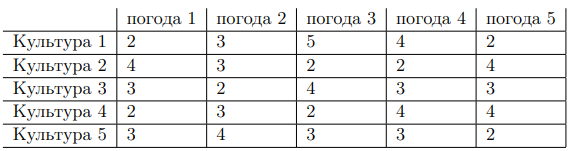
\includegraphics[width=0.75\linewidth]{image_1.png}
        
        
    \end{center}
    \item Здесь у фермера нет реального противника;
    \item Но, если фермер планирует свою деятельность в расчете на наихудшие погодные условия;
    \item Но, если фермер планирует свою деятельность в расчете на наихудшие погодные условия, то можно считать Природу активным субъектом, который пытается создать наихудшую
(с точки зрения фермера) погоду;
    \item В таком случае, мы можем смоделировать задачу фермера как матричную игру, в которой фермер является игроком 1, а Природа — игроком 2;
    \item Матрица A выигрышей в данной игре — это таблица доходов фермера.
\end{itemize}

\textbf{Задание: сведите матричную игру к задаче ЛП; создайте модель в AMPL; создайте файл данных для своего варианта; решите пример; в отчет включите файлы
и ответ} 
\begin{center}
    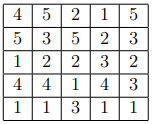
\includegraphics[width=0.25\linewidth]{image_2.png}
\end{center}
Запишем эту матрицу как задачу ЛП:
$$x_1 + x_2 + x_3 + x_4 + x_5 \rightarrow max$$
$$4x_1 + 5x_2+2x_3+x_4+5x_5 \leq 1$$
$$x_1 + 2x_2+2x_3+3x_4+2x_5 \leq 1$$
$$4x_1 + 4x_2+x_3+4x_4+3x_5 \leq 1$$
$$x_1 + x_2+3x_3+x_4+x_5 \leq 1$$
$$x_1, x_2, x_3 \geq 0.$$
Построим модель в AMPL:
\begin{center}
    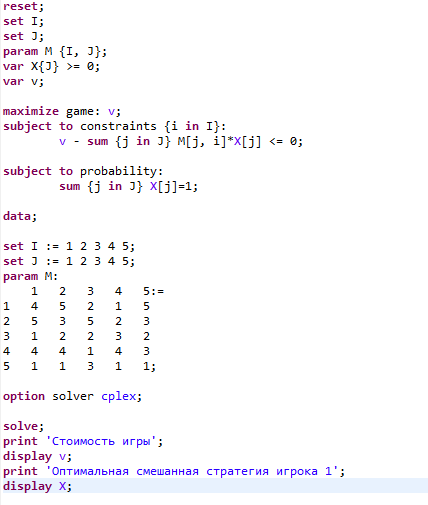
\includegraphics[width=0.75\linewidth]{image_3.png}
\end{center}
Результат работы:
\begin{center}
    
\includegraphics[width=0.5\linewidth]{image_4.png}
\end{center}
Таким образом, мы получили, что стоимость игры $v = 3$, а оптимальная смешанная стратегия игрока $I: p = [0, 0.5, 0, 0.5, 0].$
    \subsubsection*{Задание 4}

Магазин имеет некоторый запас товаров ассортиментного минимума. Если
запас товаров недостаточен, то необходимо завести его с базы; если запас
превышает спрос, то магазин несет расходы по хранению нереализованного
товара. Пусть спрос на товары лежит в пределах \(S \  5 \leq S \leq 8\)
единиц, расходы по хранению одной единицы товара составляют $c$ руб., а
расходы по завозу единицы товара \(k\) руб., цена за единицу товара
составляет \(p\) руб. Составить платежную матрицу, элементами которой
является прибыль магазина (доход от продажи с учетом расходов по
хранению или по завозу). Определить оптимальную стратегию магазина по
завозу товаров, используя критерии Вальда, Сэвиджа, Гурвица при
\(\alpha = 0.5\), Лапласа.
\begin{center}
    \begin{table}[h]
        \centering
        \begin{tabular}{|c|}
            \hline
             $p = 410, c=50, k = 80$ \\
             \hline
        \end{tabular}
    \end{table}
\end{center}

В игре участвуют 2 игрока: А – магазин, П – покупатель (природа).
Игрок А стремится реализовать свою продукцию так, чтобы получить максимальную прибыль. 

Стратегиями игрока А являются:\\
А1 – реализовывать товар в расчете на спрос в 5 единиц;\\
А2 – реализовывать товар в расчете на спрос в 6 единиц.;\\
А3 – реализовывать товар в расчете на спрос в 7 единиц;\\
А4 – реализовывать товар в расчете на спрос в 8 единиц.\\

Состояния природы П могут быть следующими:\\
П1 – спрос на товар в 5 единиц;\\
П2 – спрос на товар в 6 единиц;\\
П3 – спрос на товар в 7 единиц;\\
П4 – спрос на товар в 8 единиц.\\

Рассчитаем элементы платежной матрицы (прибыль магазина, руб.):

Стратегии игрока А

\begin{table}[h]
    \centering
    \tiny
    \begin{tabular}{|c|c|c|c|c|}
    \hline
         Стратегии & A1 & A2 & A3 & A4 \\
         \hline
         5 ед. &  $5 \cdot 410-5 \cdot 80=1650$ & $5 \cdot 410-5 \cdot 80=1650$ & $5 \cdot 410-5 \cdot 80=1650$ & $5 \cdot 410-5 \cdot 80=1650$ \\
         \hline
         6 ед. & $5 \cdot 410-(6\cdot80+1\cdot50) =1520$ & $ 6\cdot410-(6\cdot80)=1980$ & $ 6\cdot410-(6\cdot80)=1980$ & $ 6\cdot410-(6\cdot80)=1980$ \\
         \hline
         7 ед. & $5\cdot410-(7\cdot80+2\cdot50) =1390$ & $6\cdot410-(7\cdot80+1\cdot50) =1850$ & $7\cdot410-7\cdot80=2310$ & $7\cdot410-7\cdot80=2310$\\
         \hline 
         8 ед. & $5\cdot410-(8\cdot80+3\cdot50) =1260$ & $6\cdot410-(8\cdot80+2\cdot50) =1720$ & $7\cdot410-(7\cdot80+1\cdot50)=2260$ & $8\cdot410-8\cdot80=2640$\\
         \hline
    \end{tabular}
\end{table}
Окончательно, платежная матрица примет вид
\begin{table}[h]
    \centering
    \begin{tabular}{|c|c|c|c|c|}
        \hline
         Стратегии & П1 & П2 & П3 & П4 \\
         \hline
         A1 & 1650 & 1650 & 1650 & 1650 \\
         \hline
         A2 & 1520 & 1980 & 1980 & 1980 \\
         \hline
         A3 & 1390 & 1850 & 2310 & 2310 \\
         \hline 
         A4 & 1260 & 1720 & 2260 & 2640 \\
         \hline
    \end{tabular}
\end{table}
Найдем седловую точку.
$$α(A) = \max_{1\leq i \leq n} \min_{1\leq j \leq n}a_{ij} = 1650$$
$$β(A) = \min_{1 \leq j \leq n} \max_{1 \leq i \leq n}a_{ij} = 1650.$$
Соответственно мы нашли седловую точку $(1; 1)$, цена игры в этой точке $v = 1650.$ Значит, оптимальное решение $(A1; \text{П1}).$

Магазин (игрок А) получит гарантированную прибыль в размере $1650$ руб. , если будет
реализовывать свою продукцию при реализации товара в расчете на спрос в $5$ ед.
Применим различные критерии для решения задачи.

\subsubsection*{Критерий Лапласа}
Вероятность состояний природы оценивается субъективно
как равнозначные.
$$q_i =\dfrac{1}{n}$$
$$\sum q_i =
\sum \dfrac{1}{n}= 1.$$
Этот принцип называется — принцип недостаточного основания Лапласа.
В нашем случае $q_i = \dfrac{1}{4}$
\begin{table}[h]
    \centering
    \begin{tabular}{|c|c|c|c|c|c|}
        \hline
         Стратегии & П1 & П2 & П3 & П4 & $\dfrac{1}{n} \sum a_{ij}$\\
         \hline
         A1 & 1650 & 1650 & 1650 & 1650 & 1650 \\
         \hline
         A2 & 1520 & 1980 & 1980 & 1980 & 1865 \\
         \hline
         A3 & 1390 & 1850 & 2310 & 2310 & 1965\\
         \hline 
         A4 & 1260 & 1720 & 2260 & 2640 & 1970\\
         \hline
    \end{tabular}
\end{table}

Для определения оптимальной стратегии выбираем $$L = \max_{i \in \{1, ..., m\}} \dfrac{1}{n} \sum a_{ij} = 1970 \Rightarrow \textbf{Выбираем стратегию А4}.$$

\subsubsection*{Критерий Вальда}
Критерий Вальда (критерий гарантированного результата,
максиминный критерий) позволяет выбрать наибольший
элемент матрицы доходности из её минимально возможных
элементов
$$W = \max_i \min_j a_{ij}$$
Критерий Вальда предназначен для выбора из
рассматриваемых вариантов стратегий варианта с
наибольшим показателем эффективности из минимально
возможных показателей для каждого из этих вариантов.
\begin{table}[h]
    \centering
    \begin{tabular}{|c|c|c|c|c|c|}
        \hline
         Стратегии & П1 & П2 & П3 & П4 & $\min a_{ij}$\\
         \hline
         A1 & 1650 & 1650 & 1650 & 1650 & 1650 \\
         \hline
         A2 & 1520 & 1980 & 1980 & 1980 & 1520 \\
         \hline
         A3 & 1390 & 1850 & 2310 & 2310 & 1390\\
         \hline 
         A4 & 1260 & 1720 & 2260 & 2640 & 1260\\
         \hline
    \end{tabular}
\end{table}
Для определения оптимальной стратегии выбираем $$W = \max_i\min_j a_{ij} = 1650 \Rightarrow \textbf{Выбираем стратегию А1}.$$

\subsubsection*{Критерий Сэвиджа}
Критерий Сэвиджа (критерий минимаксного риска
Сэвиджа) предназначен для выбора максимального элемента
матрицы рисков из её минимально возможных элементов:
$$S = \min_i \max_j r_{ij},$$ где $$r_{ij} = \max_ia_{ij} - a_{ij}.$$
Построим матрицу рисков
\begin{table}[h]
    \centering
    \begin{tabular}{|c|c|c|c|c|c|}
        \hline
         Стратегии & П1 & П2 & П3 & П4 & $\max r_{ij}$\\
        \hline
         A1 & 0 & 330 & 660 & 990 & 990\\
         \hline
         A2 & 130 & 0 & 330 & 660 & 660\\
         \hline
         A3 & 260 & 130 & 0 & 330 & 330 \\
         \hline
         A4 & 390 & 260 & 50 & 0 & 390\\
         \hline
    \end{tabular}
\end{table}

Для определения оптимальной стратегии выбираем $$S = \min_i \max_j r_{ij} = 330 \Rightarrow \textbf{Выбираем стратегию А3}.$$

\subsubsection*{Критерий Гурвица.}
Критерий Гурвица (взвешивает пессимистический и
оптимистический подходы к анализу неопределенной
ситуации) предназначен для выбора некоторого среднего
элемента матрицы доходности, отличающегося от крайних
состояний – от минимального и максимального элементов:
$$H = \max_i {(} λ \cdot \max_j a_{ij} + {(}1 - λ{)} \cdot \min_j a_{ij}{)}, $$
где $λ$ — коэффициент оптимизма, $0 \leq λ \leq 1$, в нашем случае он равен $\lambda = 0.5$.
\begin{table}[h]
    \centering
    \begin{tabular}{|c|c|c|c|c|c|}
        \hline
         Стратегии & П1 & П2 & П3 & П4 & $ 0.5 \cdot \max_j a_{ij} + 0.5 \cdot \min_j a_{ij}$\\
         \hline
         A1 & 1650 & 1650 & 1650 & 1650 & 1650 \\
         \hline
         A2 & 1520 & 1980 & 1980 & 1980 & 1750 \\
         \hline
         A3 & 1390 & 1850 & 2310 & 2310 & 1850\\
         \hline 
         A4 & 1260 & 1720 & 2260 & 2640 & 1950\\
         \hline
    \end{tabular}
\end{table}

Для определения оптимальной стратегии выбираем $$H = \max_i {(} λ \cdot \max_j a_{ij} + {(}1 - λ{)} \cdot \min_j a_{ij}{)} = 1950 \Rightarrow \textbf{Выбираем стратегию А4}.$$
\end{document}
